\documentclass[12pt]{article}

\usepackage{graphicx}

\title{Color-Magnitude Diagram of M37}
\date{2016 May 26}
\author{Brendon Walter}

\begin{document}
	\maketitle
	
	\section{Abstract}
		Images of M37 were taken with CCD on a 16 inch telescope on Bennington College campus. Image correction was done and two final images, one in a blue filter and one in green were created. Aperture photometry was preformed on these two images with 590 stars in the field being identified, analyzed, and plotted. The resulting Color-Magnitude Diagram has a very clear main sequence, although many of the stars in the image don't seem to fall it, or any of the other expected branches. However, there is a clump of stars to the upper right of the main sequence around where the red giant branch is expected, although it is lower than anticipated.
	
	\section{Introduction}
		Messier 37 - often referred to simply as M37 - is an open cluster in the constellation Auriga and was discovered by Giovanni Hodierna by 1654 and was later cataloged by Charles Messier in 1764. Over 500 stars have been confirmed to be in the cluster and it is around 90 light years in diameter. It is 4,500 light years away from Earth. [1]
		\\\\
		A Color-Magnitude Diagram, or a CMD, is a version of what's commonly known as an H-R Diagram which plots the luminosity of stars vs. their temperature. Most (85\%) of stars are found on what's known as the main sequence, primarily because this is the region in which a star spends most of its life in. A star's position on the main sequence is determined by the mass of the star. As the star ages it will move off the main sequence and into the red giant or supergiant branch, which can be found on the upper right of the main sequence. 
		\\\\
		In a CMD, the color of the star acts as a proxy for temperature and the brightness a proxy for luminosity. This makes it easier to make a chart comparing these values rather than measuring and calculating the temperature and luminosity for each star - a task which can sometimes be impossible. As the brightness of a star can vary by its distance from earth, a CMD is only useful when it comes to looking at star clusters because each star in the cluster is more or less at the same distance from Earth and any variation in distance between stars will be very slight.
		\\\\
		Looking at the point at which stars are moving off the main sequence and into the red giant branch says something about how old the cluster is - if the main sequence is fairly long, most of the stars are still in the main part of their life and so it can be argued the the cluster is fairly young. As the main sequence turnoff point becomes shorter, it can be reasoned the the cluster is older.
		
		
	\section{Data Collection}
		\subsection{Imaging}
			Images were taken using a CCD on the 16 inch telescope at the Stickney Observatory on Bennington College campus. The images were taken on March 30 starting at 4:15 am UT and were taken over a 40 minute time frame Eight total images of M37 were used, four taken using a green filter and the other four using a blue filter. These filters were chosen because the difference in the magnitude in the visual spectrum from the magnitude in the blue (B-V value) is correlated with stellar temperatures. As we do not posses a visual filter, a green filter was used in its place.
			\\\\
			Twilight sky flats were taken the next night, March 30, as the equipment was failed to be set up in time the night the observations were made. 
	
		\subsection{Processing}
			Dark and bias images were automatically removed from the images of M37 as they were taken by Maxim DL. Images were then flat corrected using AstroImageJ. Once the images were cleaned up, the images were aligned and stacked by AstroImageJ into two final images to remove noise - one of the cluster in the blue filter (Fig. 1) and one of it in the green.
	
		\begin{figure}
			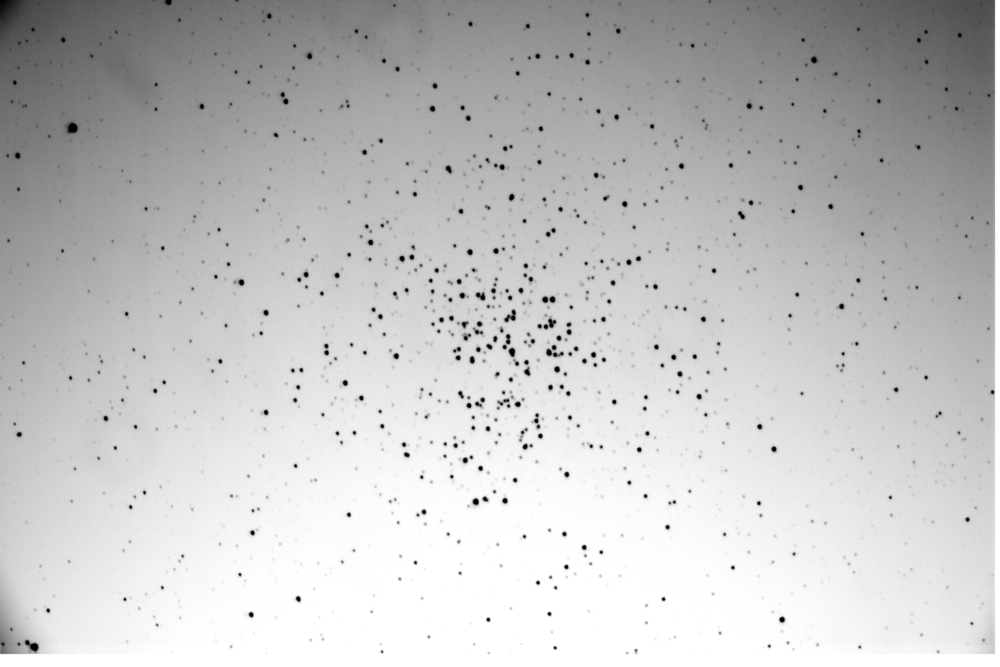
\includegraphics[width=\textwidth]{./images/MED_aligned_B.png}
			\caption{Processed and stacked image of M37 in the blue filter. Images were taken over a 40 minutes period on March 30 starting around 4:15 am UT.}
		\end{figure}
		
		\begin{figure}
			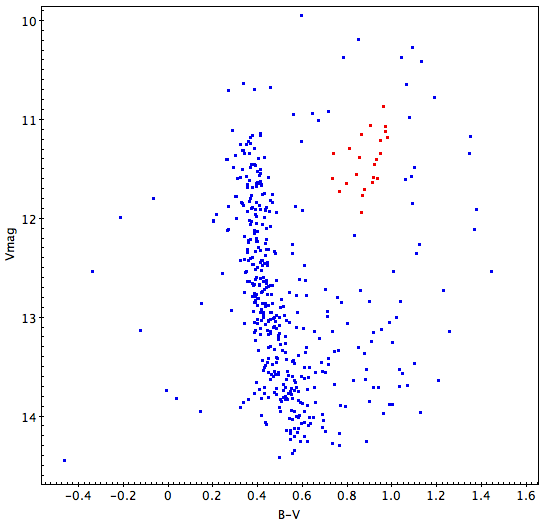
\includegraphics[width=\textwidth]{./images/cmd.png}
			\caption{CMD of M37, plotting brightness in the green compared to color. The main sequence is very clear and well defined and the stars highlighted in red on the upper right are probable red giants.}
		\end{figure}	
					
		\begin{figure}
			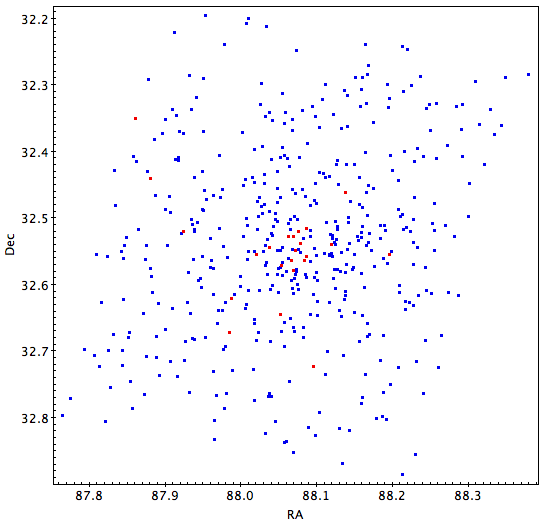
\includegraphics[width=\textwidth]{./images/redgiants.png}
			\caption{Positions (in Right Ascension and Declination) of the analyzed stars in the star cluster. The red stars are the same probable red giants highlighted in the CMD above. The fact that they seem to be more densely packed in the center of the cluster says that they are likely associated with the cluster and so are likely red giants.}
		\end{figure}
	
		\subsection{Data Extraction}
			Aperture photometry was then preformed on the two final, stacked images of the star cluster. Aperture sizes were chosen based off the Full Width at Half Max (FWHM) of a star chosen at random in the frame. APT was able to automatically find and place apertures around 600 stars in the blue image and 590 in the green. Sky noise was subtracted using the sky-annulus median subtraction option offered by APT. TopCAT was then used to process and calibrate the data in table format, calculate the B-V value (where the green magnitude was used in place of the visual value) for each star, and then create charts of the star cluster (Figs. 2 and 3).
	
	\section{Analysis \& Discussion}
		There is a very clear main sequence branch in the resulting CMD (Fig. 2). Stars in this range have an apparent green magnitude ranging from 14.5 to 11, with lower values being brighter. They have B-V values ranging from around 0.3 to 0.7, with lower values correlating with higher temperatures.
		\\\\
		Many of the stars in the image don't seem to fall into the main sequence or any of the other expected branches. This may be because 590 stars were auto-identified by APT whereas there are only around 500 stars confirmed to be a part of the cluster. Thus, many of these stars may be stars that are not actually a part of the cluster and thus do not fall correctly into the CMD.
		\\\\
		However, there is a clump of stars to the upper right of the main sequence, highlighted in red in Fig. 2. This clump has more of a  shape to it and is around where the red giant branch is expected to be found. To confirm this, the suspected stars were plotted against every other star by position in the cluster (Fig. 3). If these stars are a part of the cluster, it is expected that there would be a higher density of these possible red giants in the center of the cluster. Indeed, this seems to be the case and so it is likely that these stars are red giants.
		\\\\
		The red giant branch is, however, lower down on the y-axis than is expected. As red giants were main sequence stars that have moved off the main sequence as they aged, it's expected that the the start of the red giant branch would correlate more with the end of the main sequence. A possible future, follow up project would be to look at these 'blue stragglers' and see if they are systems with multiple stars in them which could give an inaccurate understanding of the luminosity and color of these stars when viewed in this kind of setting.
		
	
	\section{Areas of Difficulty}
		Several issues were ran into when taking the images of M37. The flat field images were very faint and, while better than not flat correcting at all, it's questionable as to how cleaned up the images actually are. Another issue was that M37 was fairly low on the horizon when these images were taken, meaning that the telescope was looking through a lot more atmosphere than is ideal. 
		\\\\
		Additionally, images that were taken in the green filter should have been taken in the visual filter in order to give a more accurate B-V value. Unfortunately, we do not own a visual filter and so a green filter had to be used in its place. As a result, the B-V values are not as insightful as they would be otherwise.
	
	\section{Citations}
		\begin{enumerate}
			\item "Messier 37." Messier Objects. N.p., 30 Apr. 2015. Web. 25 May 2016. 
			\\http://www.messier-objects.com/messier-37/
			\item Pogge, Richard. "Lecture 10: Synthesis: The Hertzsprung-Russell Diagram." Lecture 10: The H-R Diagram. N.p., 3 May 2008. Web. 25 May 2016. 
			\\ http://www.astronomy.ohio-state.edu/~pogge/Ast162/Unit1/hrdiag.html
		\end{enumerate}
	
\end{document}